% +------------------------------------------------------------------------+
% | CGAL User Manual:  reference.tex
% +------------------------------------------------------------------------+
% | R-tree User Manual
% |
% | 31.03.2000   Gabriele Neyer
% |              Start writing the user manual
% | 
\RCSdef{\hdsRev}{$Revision$}
\RCSdefDate{\hdsDate}{$Date$}
% +------------------------------------------------------------------------+

\section{Software Engineering Perspectives}

%\begin{ccTexOnly}
%\begin{figure}
%%\psfrag{A}{\footnotesize\ccc{Data}}
%%\psfrag{B}{\footnotesize\ccc{Key}}
%%\psfrag{C}{\footnotesize\ccc{R_tree_traits}}
%%\psfrag{D}{\footnotesize\ccc{R_tree}}
%%\psfrag{E}{\footnotesize\ccc{IO_tree_traits}}
%%\psfrag{F}{\footnotesize\ccc{IO_tree_traits}}
%%\psfrag{G}{\footnotesize\hspace*{-.1cm}\parbox{1.9cm}{Database of tree nodes}}
%%\psfrag{H}{\footnotesize\hspace*{-.1cm}\parbox{1.9cm}{Database of leaf nodes}}
%%\psfrag{I}{\footnotesize\ccc{choose_subtree}}
%%\psfrag{J}{\footnotesize\ccc{split_node}}
%%\psfrag{K}{\footnotesize\ccc{split_leaf}}
%%\psfrag{L}{\footnotesize\ccc{reinsertion_node}}
%%\psfrag{M}{\footnotesize\ccc{reinsertion_leaf}}
%%\psfrag{O}{\footnotesize\ccc{R_tree_index}}
%%\psfrag{P}{\footnotesize\ccc{R_tree_storage}}
%\begin{center}
%\includegraphics[width=14cm,clip]{rtree-classes4.eps}
%\end{center}
\%caption{\label{r-tree-design} R-Tree components}
%\end{figure}
%\end{ccTexOnly}
%\begin{ccHtmlOnly}
%    <!2><TABLE BORDER=0 CELLSPACING=2 CELLPADDING=0 WIDTH=650>
%        <TR><TD ALIGN=LEFT VALIGN=TOP WIDTH=100% NOWRAP COLSPAN=2>
%    <img border=0 src="./rtree-classes4.gif" alt="R-Tree components">
%    </TD>
%    <TD ALIGN=LEFT VALIGN=TOP WIDTH=50%><img border=0 src="./rtree-classes4.gif"
%alt="R-Tree components">
%      </TD></TR></TABLE>
%\end{ccHtmlOnly}
%
%\begin{ccTexOnly}
%Figure~\ref{r-tree-design} shows the different components of the
%R-Tree (R$^\star $-Tree) that can be plugged into the tree. 
%\end{ccTexOnly}
%\begin{ccHtmlOnly}
%Figure~\ref{r-tree-design} shows the different components of the
%R-Tree (R$^\star $-Tree) that can be plugged into the tree. 
%\end{ccHtmlOnly}
The R-Tree has three template arguments (see the figure above). 
The \ccc{R-tree_traits}
class which defines the data handling, the \ccc{R_tree_index}
class which defines all \ccc{index} strategies and one traits
class which defines the databases and sizes of the tree nodes and
leaves. This class is called \ccc{R_tree_storage}. We now
describe each component more in detail. Note,
for
each component CGAL provides example classes or implementations
of the most important or most commonly used strategies.

\subsubsection{Data handling}
In this section we describe how data is handled in the tree.
\medskip

\noindent
{\bf Tree Data}\\
\noindent
The tree is designed to handle arbitrary spatial objects (called
\ccc{Data}) in arbitrary dimensions.
Each node of the tree stores a \ccc{Key} which usually is the
bounding box of the \ccc{Key}s of its childs. The tree is designed to be
independent of the form of a \ccc{Key}. 
That is a \ccc{Key} can have arbitrary dimension and arbitrary
form (e.g. a $d$-dimensional bounding box, the smallest enclosing
$d$-dimensional ball, etc). Nevertheless, the \ccc{Key} class has
to provide certain properties: 
E.g. for two \ccc{Key}s it must be decidable if one \ccc{Key} is contained in
the other one, if they intersect and what the smallest \ccc{Key}
is that encloses both \ccc{Key}s.
Besides access functions a \ccc{cost}-function has to be provided
that measures the inefficiency when clustering two \ccStyle{Key}s
together. This allows the user to build the R-Tree in respect to
different optimization functions such as minimum area, overlap or
margin enlargement when clustering two \ccStyle{Key}s together.
CGAL provides predefined
\ccc{Key} classes for $k$-dimensional aligned rectangles, $1\le k\le
4$ (see Section~\ref{k-key}). 
A traits class implementation that defines all necessary functions is
described in Section~\ref{interface}. 
\medskip

\noindent
{\bf R\_tree\_traits}\\
\noindent
The \ccc{Data}
and \ccc{Key} functionality is
accessed through a traits class we call \ccc{R_tree_traits}. This traits class decouples
the R-tree  from the \ccc{Data}
and \ccc{Key} class such that a modification of one of these classes
only affects this traits class but not the tree. 
The \ccc{R_tree_traits} class requirements are
described in  Section~\ref{interface}.
\cgal\ provides a predefined \ccc{R_tree_traits} class for the
predefined \ccc{Key} classes (see Section~\ref{Rtreetraitspre}). 
%The
%spatial objects are spatially clustered in the tree according to
%their orthogonal bounding boxes (called \ccStyle{Key}, see
%Section~\ref{k-key}).  A \ccStyle{Key} usually is a
%$k$-dimensional aligned rectangle, but it is also possible to
%define a different geometric object as \ccStyle{Key}. 



%The \ccc{cost}-function determines the cost of one key or the cost
%that arises when two keys are put together. The tree accesses the
%\ccc{cost}-function through a traits class and is therefore
%independent of the specific cost function.
%The user has to provide
%key specific functions that measure if two keys intersect,
%compute a penalty cost when clustering two keys together,
%etc. 

\subsubsection{R\_tree\_index}
The R-Tree index defines how the data is spatially clustered in
the tree. We decoupled the index strategies from the
implementation of the tree since many diffrent index
strategies have been proposed for the R-Tree. \cgal\ provides two 
\ccc{R_tree_index} classes that can be plugged into the tree: The
\ccc{R_tree_index} class which is the index strategy as
proposed by Guttman~\cite{gutt-84} and the \ccc{R_star_tree_index}
class which is the R$^\star$-Tree index strategy as proposed by  Beckmann
et al~\cite{Beckmann:1990:RER} (see Section~\ref{preindex}). The
requirements for a user defined \ccc{R_tree_index} class are
given in Section~\ref{indexreq}.
We here give a
short description of the index strategies.
\medskip

\noindent
{\bf choose\_subtree}\\
\noindent
In the \ccc{choose-subtree} strategy a subtree is chosen in which 
the new element is to be inserted. 
%Many \ccc{choose-subtree}
%strategies have been proposed. We therefore decoupled this
%strategy from the implementation of the R-Tree. 
We implemented
the \ccc{choose-subtree} strategy from Guttman~\cite{gutt-84}
and from Beckmann
et al~\cite{Beckmann:1990:RER} which can be plugged into the
tree (see Section~\ref{Choosepre}). The requirements for a user
defined \ccc{choose-subtree} strategy are given in
Section~\ref{userchoose}.
\medskip

\noindent
{\bf split\_node and split\_leaf}\\
\noindent
%Since many merging and splitting strategies have been proposed
%for the R-Tree and the R$^\star$-Tree we decoupled these strategies from the
%implementation of the R-Tree. 
The \ccc{split_node} and \ccc{split_leaf} method distributes the
entries of an overfilled inner node, resp. leaf, into two.
We implemented some important splitting
strategies like those from Guttman~\cite{gutt-84} and Beckmann
et al~\cite{Beckmann:1990:RER} which can be plugged into the
tree (see Section~\ref{Splitpre})
Note that one can plug in a different split strategy for the
inner nodes as for the leaf nodes of the tree.
See Section~\ref{userchoose} for the 
requirements a user implemented split strategy has to fulfill.
\medskip

\noindent
{\bf reinsertion\_node and reinsertion\_leaf}\\
\noindent
The R$^\star$-Tree forces entries to be reinserted during the
insertion routine. 
In the \ccc{reinsertion_node} and \ccc{reinsertion_leaf} method,
an overfilled node is divided into two parts. The one part stays
in that node and the other part is reinserted into the same level 
of the tree as the node is.
%Sine different reinsertion strategies have
%been proposed we decoupled these strategies from the
%implementation of the R-Tree. 
We implemented the
\ccc{close_reinsert} reinsertion
strategy of  Beckmann
et al~\cite{Beckmann:1990:RER} which can be plugged into the
tree. See Section~\ref{Reinsertpre} for the implementations of
the reinsertion strategies and  Section~\ref{userreinsert} for the
requirements a user implemented reinsertion strategy has to fulfill.
\medskip

\noindent
{\bf reinsertion}\\
\noindent
\label{reinsertion} 
The \ccc{R_tree_index} class gets a boolean template
  argument \ccc{reinsertion}. In case \ccc{reinsertion=true}
  entries are reinserted during the insertion process. More
  precisely, let a node be overfilled. Then, a part of the
  entries of this node is reinserted in case that no reinsertion 
  in the level of the node has been performed before. The entries 
  that are to be reinserted are chosen in the \ccc{reinsertion_node}
  class, \ccc{reinsertion_leaf} class, resp. Otherwise, a split is 
  performed. Note, the leaf level is the level number 0.

\subsubsection{R\_tree\_storage}
The \ccc{R_tree_storage} class  is a traits class in which all
storage dependant components of the R-Tree are defined. These are 
a database for the laef nodes, a database for the inner nodes of
the tree, the capacities of the nodes in form of the number of
elements and the size of a page, etc. \cgal\ provides two
predefined \ccc{R_tree_storage} classes called
\ccc{R_tree_internal_storage} and \ccc{R_tree_external_storage}
that can be plugged into the tree (see
Section~\ref{prestorage}). For the requirements of a user defined 
storage class see Section~\ref{storagereq}.
We now give a short description of the components of the
\ccc{R_tree_storage} class. 
\medskip

\noindent
{\bf Databases}\\
\noindent
The R-Tree has two databases. One for the inner nodes of the tree
and one for the leaf nodes. 

Each database is decoupled from the \ccc{R_tree_storage} class
 by an \ccc{IO_traits} 
class. %Both databases have to provide the same basic functionality. 
%We provide an I/O traits class that specifies the
%necessary functionality of a database (see Section~\ref{IOpre}). 
\cgal\ provides two databases for the R-Tree (see
Section~\ref{IOpre}). 
One stores the data and the tree in
internal memory. 
The other database  is an external memory database which
allocates a memory cache for $k$ pages of size pagesize, whereby $k$ is an
integer template argument. The cache uses the least recently used
strategy to load and unload pages. Note that other
databases  
can be plugged into the tree by providing an appropriate \ccc{IO_traits}
class. See Section~\ref{userIO} for the requirements a user
implemented database must fulfill.
\medskip

\noindent
{\bf Node and Leaf Capacities}\\
\noindent
The \ccc{R_tree_storage} class gets 4 integer template arguments.
The  minimum
capacity (\ccc{IO_min_cap_nodes}) and
maximum capacity (\ccc{IO_max_cap_nodes}) has to be defined for
an inner node of the tree.
Each inner node is guaranteed to have between \ccc{IO_min_cap_nodes} and
\ccc{IO_max_cap_nodes} \ccc{Key} entries; the root node has between 2 and
\ccc{IO_max_cap_nodes} entries. 
For the leaf nodes \ccc{IO_min_cap_leaves} defines the minimum
number of elements in a leaf and \ccc{IO_page_size} defines the maximum size of
all \ccc{Data} entries of a leaf.
\medskip

\noindent
{\bf headerextern}\\
\noindent
\ccc{headerextern} is a boolean template argument.
In case \ccc{header_extern=true}
  a header file containing necessary informations for the
  reconstruction of a tree from an external database is stored on
  disk. Otherwise, the header file is not stored on disk.

\subsubsection{More Features}
\begin{description}
\item[reinsertion control]
For each level of the tree, a reinsertion flag can be set to \ccc{true} 
or \ccc{false}. In case that the reinsertion flag of a level is
true, the \ccc{reinsertion_node} (\ccc{reinsertion_leaf} resp.)
routine will be called for an overfull node of this level (instead 
of the split routine). When the \ccc{reinsertion_node}
(\ccc{reinsertion_leaf} resp.) routine is finished, the
reinsertion flag is again set to \ccc{false} for that level.
See Section~\ref{r-tree} for a description 
of the functions \ccc{get_reinsertion_flag} and \ccc{set_reinsertion_flag}.
\item[output sensitive query function]
The query functions are output sensitive. That is, we
provide iterators that allow to intermix user code with
querying. Since the amount of query output can exceed
the main memory capacity there is no alternative than providing
output sensitive query functions (see Section~\ref{r-tree}).
\end{description}


%The implementation of the R-Tree follows the design issues of the
%generalized search tree~\cite{Hellerstein}. That is, the tree is designed
%to handle  arbitrary geometric objects (called \ccStyle{Data}) in
%arbitrary dimension. The traits class for the \ccc{Data} is
%described in  Section~\ref{data}. The
%spatial objects are spatially clustered in the tree according to
%their orthogonal bounding boxes (called \ccStyle{Key}, see
%Section~\ref{k-key}).  A \ccStyle{Key} usually is a
%$k$-dimensional aligned rectangle, but it is also possible to
%define a different geometric object as \ccStyle{Key}. CGAL provides predefined
%key classes for $k$-dimensional aligned rectangles, $1\le k\le
%4$. The user has to provide
%key specific functions that measure if two keys intersect,
%compute a penalty cost when clustering two keys together,
%etc. A traits class that defines all necessary functions is
%described in Section~\ref{interface}. This traits class is
%implemented out for the predefined key classes.
%The split strategies and the requirements for user
%defined split strategies are given in Section~\ref{split}.
%Since the split strategies work on predefined classes that
%contain either a key or a data element and some additional
%information on these elements, these classes are defined in Section~\ref{cont}.
%The definition of the \ccStyle{R_tree} is given in
%Section~\ref{r-tree}. In the end of this chapter an example is given.

%%%%%%%%%%%%%%%%%%%%%%%%%%%%%%%%%%%%%%%%%%%%%%%%%%%%%%%%%%%%%%%%%%%%%
%%%%%%%%%R-TREE%%%%%%%%%%%%%%%%%%%%%%%%%%%%%%%%%%%%%%%%%%%%%%%%%%%%%%
\section{R-Tree Class}
\label{r-tree}
\begin{ccClassTemplate}{R_tree<R_tree_traits, R_tree_index, R_tree_storage>}

\noindent
{\bf Class: R\_tree$<$R\_tree\_traits, R\_tree\_index, R\_tree\_storage$>$}

\ccDefinition
The R-Tree gets 3 template arguments.
\begin{description}
\item[\ccc{R_tree_traits}] This class builds the interface to the 
  \ccc{Data} and \ccc{Key}s of the tree. The requirements of this 
  class are defined in Section~\ref{treetraitsreq}. A predefined
  \ccc{R_tree_traits} class is described in
  Section~\ref{Rtreetraitspre}.
\item[\ccc{R_tree_index}] This class is a traits class in which
  the index strategies (\ccc{choose_subtree, split_node,
    split_leaf, reinsertion_node, reinsertion_leaf}) are
  defined. \cgal\ provides two predefined index traits classes
  (see Section~\ref{preindex}). The requirements for a user defined 
  index class are given in Section~\ref{indexreq}.
\item[\ccc{R_tree_storage}] This class is a traits class in which 
  the storage depending components are defined.  These are 
a database for the laef nodes, a database for the inner nodes of
the tree, the capacities of the nodes in form of the number of
elements and the size of a page, etc. \cgal\ provides two
predefined \ccc{R_tree_storage} classes called
\ccc{R_tree_internal_storage} and \ccc{R_tree_external_storage}
that can be plugged into the tree (see
Section~\ref{prestorage}). For the requirements of a user defined 
storage class see Section~\ref{storagereq}.
%\item[\ccc{Choose_subtree}] This class provides an \ccc{operator()} member
%function which gets all entries of a node, and a \ccc{Key} of
%a \ccc{Data} entrie that has to be inserted. It returns a node
%entrie that specifies the subtree in which the new \ccc{Data}
%entrie is to be inserted.  The requirements of this 
%  class are defined in Section~\ref{userchoose}. Predefined
%  \ccc{Choose_subtree} classes are described in Section~\ref{Choosepre}.
%\item[\ccc{Split_node}] An overfilled inner node of the tree is
%  split according to the split strategy that is defined in this
%  class. The requirements of this 
%  class are defined in Section~\ref{usersplit}. Predefined
%  \ccc{Split_node} classes are described in Section~\ref{Splitpre}.
%\item[\ccc{Split_leaf}] An overfilled leaf of the tree is
%  split according to the split strategy that is defined in this
%  class. The requirements of this 
%  class are defined in Section~\ref{usersplit}. Predefined
%  \ccc{Split_leaf} classes are described in Section~\ref{Splitpre}.
%\item[\ccc{Reinsertion_node}] In case that a part of an overfilled
%inner node is reinserted, the \ccc{reinsertion_node} strategy, which is
%defined in this class, is called. It computes the set of entries
%that is to be reinserted. The requirements of this 
%  class are defined in Section~\ref{userreinsert}. Predefined
%  \ccc{Reinsertion_node} classes are described in
%  Section~\ref{Reinsertpre}.
%\item[\ccc{Reinsertion_leaf}] In case that a part of an overfilled
%inner leaf is reinserted, the \ccc{reinsertion_leaf} strategy, which is
%defined in this class, is called. It computes the set of entries
%that is to be reinserted. The requirements of this 
%  class are defined in Section~\ref{userreinsert}. Predefined
%  \ccc{Reinsertion_leaf} classes are described in Section~\ref{Reinsertpre}.
%\item[\ccc{IO_tree_traits_nodes}] This class specifies the
%  database for the inner nodes of the tree. The requirements of this 
%  class are defined in Section~\ref{userIO}. Predefined
%  \ccc{IO_tree_traits_node} classes are described in
%  Section~\ref{IOpre}.
%\item[\ccc{IO_tree_traits_leaf}] This class specifies the
%  database for the leaf nodes of the tree. The requirements of this 
%  class are defined in Section~\ref{userIO}. Predefined
%  \ccc{IO_tree_traits_leaf} classes are described in Section~\ref{IOpre}.
%\item[\ccc{IO_pagesize}] This integer template argument specifies 
%  the size of a page. The tree and leaf data is stored in disk
%  blocks of this size.
%This size must be smaller than a third of the
%  size of the
%  internal memory such that at least three pages can be kept in
%  internal memory without swapping.
%\item[\ccc{header_extern}] The R-Tree gets a boolean template
%  argument \ccc{header_extern}. In case \ccc{header_extern=true}
%  a header file containing necessary informations for the
%  reconstruction of a tree from an external database is stored on
%  disk. Otherwise the header file is not stored on disk.
\end{description}
\ccInclude{CGAL/R_tree.h}


\ccCreationVariable{R}


\ccCreation
\ccConstructor{R_tree();}{An empty R-Tree is constructed.}
\ccConstructor{R_tree(char *header_file, char *node_data_file,
  char *leaf_data_file);}{An R-Tree is initialized. In case that
  the \ccc{header_file} is not empty, the tree expects that
  \ccc{header_file}, \ccc{node_data_file} and
  \ccc{leaf_data_file} are files that were generated by the same
  type of R-Tree as this type is. That is, all template classes
  have to be identic. Furthermore, the files must belong
  together. In this case, the tree is build according to the data 
  in the files. Otherwise, if \ccc{header_file} is an empty file, 
  an empty tree is constructed.}

\ccOperations

%\ccMethod{void ~R_tree();}{The R-Tree is destructed. The databases are 
%  closed.}

%\ccMethod{void open(char *header_file, char *node_data_file,
%  char *leaf_data_file);}{An R-Tree is initialized. In case that
%  the \ccc{header_file} is not empty, the tree expects that
%  \ccc{header_file}, \ccc{node_data_file} and
%  \ccc{leaf_data_file} are files that were generated by the same
%  type of R-Tree as this type is. That is, all template classes
%  have to be identic. Furthermore, the files must belong
%  together. In this case, the tree is build according to the data 
%  in the files. Otherwise, if \ccc{header_file} is an empty file, 
% an empty tree is constructed.}

\ccMethod{void insert(Data& elem);}{A new element is inserted into 
  the tree.}

\ccMethod{bool find_key_include(Key a);}{If the tree contains a
  \ccc{Data} element that is contained in \ccc{Key a}, then \ccc{true} is
  returned. Otherwise, \ccc{false} is returned.}

\ccMethod{bool find_key_intersect(Key a);}{If the tree contains a
  \ccc{Data} element with a \ccc{Key k} that has non empty
  intersection with \ccc{Key a}, then \ccc{true} is
  returned. Otherwise, \ccc{false} is returned.}

\ccMethod{bool delete_key(Key& a, Data& elem);}{If the tree
  contains a \ccc{Data} element with \ccc{Key a}, then \ccc{elem} is
  set to this \ccc{Data} element and true is returned. Otherwise, 
  false is returned. Note, only one \ccc{Data} element with
  \ccc{Key a} is deleted. In order to delete another element with
  \ccc{Key a} you have to repeat the function call.}

\ccMethod{int get_rootlevel();}{The level of the root is returned.}

\ccMethod{bool get_reinsertion_flag(int the_level);}{The
  reinsertion flag of \ccc{the_level} is returned.}

\ccMethod{bool set_reinsertion_level(unsigned int the_level,bool
  value);}{The reinsertion flag of level \ccc{the_level} is set
  to \ccc{value}. If \ccc{value=true} then a part of an overfilled node in
  level \ccc{the_level} will be reinserted.}

\ccMethod{void dump();}{The tree is dumped in a readable way to \ccc{stderr}.}


\ccMethod{R_tree::iterator begin_intersect();}{An forward
  iterator that iterates through all \ccc{Data} elements of the
  tree is initialized and returned. In
  order to iterate through all elements of the tree you should
  compare your actual iterator with the \ccc{end_intersect()}
  iterator. If both iterators are identical, you reached past the
  last 
  element.}

\ccMethod{R_tree::iterator end_intersect();}{An forward
  iterator that iterates through all \ccc{Data} elements of the
  tree is initialized with the last element and returned. In
  order to iterate through all elements of the tree you should
  compare your actual iterator with the \ccc{end_intersect()}
  iterator. If both iterators are identical, you reached past the last 
  element.}

\ccMethod{R_tree::iterator begin_intersect(Key k);}{An forward
  iterator that iterates through all \ccc{Data} elements of the
  tree that have non empty intersection with \ccc{Key k} is
  initialized 
  and returned. In
  order to iterate through all elements of the tree  that have
  non empty intersection with \ccc{Key k}  you should
  compare your actual iterator with the \ccc{end_intersect(k)}
  iterator. If both iterators are identical, you reached past the last 
  element.}

\ccMethod{R_tree::iterator end_intersect(Key k);}{An forward
  iterator that iterates through all \ccc{Data} elements of the
  tree that have non empty intersection with \ccc{Key k} is
  initialized  with the last element and returned. In
  order to iterate through all elements of the tree that have non 
  empty intersection with \ccc{Key k} you should
  compare your actual iterator with the \ccc{end_intersect(k)}
  iterator. If both iterators are identical, you reached past the last 
  element.}

\ccMethod{R_tree::iterator begin_enclose(Key k);}{An forward
  iterator that iterates through all \ccc{Data} elements of the
  tree that enclose \ccc{Key k} is
  initialized 
  and returned. In
  order to iterate through all elements of the tree  that enclose
  \ccc{Key k}  you should
  compare your actual iterator with the \ccc{end_enclose(k)}
  iterator. If both iterators are identical, you reached past the last 
  element.}

\ccMethod{R_tree::iterator end_enclose(Key k);}{An forward
  iterator that iterates through all \ccc{Data} elements of the
  tree that enclose \ccc{Key k} is
  initialized  with the last element and returned. In
  order to iterate through all elements of the tree that enclose
   \ccc{Key k} you should
  compare your actual iterator with the \ccc{end_enclose(k)}
  iterator. If both iterators are identical, you reached past the last 
  element.}

\ccMethod{R_tree::iterator begin_compare(Key k);}{An forward
  iterator is initialized and returned. It iterates through all 
  \ccc{Data} elements $a$ of the
  tree for which \ccc{R_tree_traits::compare(Key k,a)=true}
  and for all \ccc{p(a)} \ccc{R_tree_traits::compare(Key k,p(a))=true},
  whereby \ccc{p(a)} is a key of an ancestor of \ccc{a} in the
  tree. In 
  order to iterate through all elements of the tree  that compare 
  with 
  \ccc{Key k}  you should
  compare your actual iterator with the \ccc{end_compare(k)}
  iterator. If both iterators are identical, you reached past the last 
  element. Note that the \ccc{compare} function is no where else used in
  the tree than for this search. Therefore, you can freely define 
  what kind of comparison is to be done.}

\ccMethod{R_tree::iterator end_compare(Key k);}{An forward
  iterator  is
  initialized  with the last element and returned.
It iterates through all 
  \ccc{Data} elements $a$ of the
  tree for which \ccc{R_tree_traits::compare(Key k,a)=true}
  and \ccc{R_tree_traits::compare(Key k,p(a))=true},
  whereby \ccc{p(a)} is a key of an ancestor of \ccc{a} in the
  tree.
  In order to iterate through all elements of the tree that
  compare with
   \ccc{Key k} you should
  compare your actual iterator with the \ccc{end_compare(k)}
  iterator. If both iterators are identical, you reached past the last 
  element.
Note that the \ccc{compare} function is no where else used in
  the tree than for this search. Therefore, you can freely define 
  what kind of comparison is to be done.}

\end{ccClassTemplate}

\begin{ccClass}{R_tree::iterator }

\noindent
{\bf Class: R\_tree::iterator}

\ccDefinition
Defines an iterator over R-Tree \ccc{Data} objects.

\ccCreationVariable{I}


\ccCreation

\ccConstructor{R_tree::iterator();}{}


\ccOperations

\ccMethod{bool operator==(R_tree::iterator & x);}{Let the
  iterators point on the \ccc{Data} elements \ccc{a} and \ccc{b}. 
  Then, \ccc{R_tree_traits::equal_data(a,b)} is returned.}
\ccMethod{bool operator!=(R_tree::iterator& x);}{Let the
  iterators point on the \ccc{Data} elements \ccc{a} and \ccc{b}. 
  Then, \ccc{!R_tree_traits::equal_data(a,b)} is returned.}
\ccMethod{R_tree::iterator& operator=(R_tree::iterator x);}{The
  iterator is set to iterator \ccc{x}.}
\ccMethod{Data operator*();}{The \ccc{Data} element the iterator
  points to is returned.}
\ccMethod{bool is_valid();}{Returns \ccc{true}, if the iterator
  points on a valid \ccc{Data} element.}
\ccMethod{R_tree::iterator& operator++();}{Depending on the query 
  function (intersection, enclose, compare), the iterator is moved
  to the next element that matches the query in respect to the 
  \ccc{Key} the iterator was initialized with.}
\ccMethod{void operator++(int );}{Same as calling \ccc{operator++()}.}

\end{ccClass}


%%%%%%%%%%%%%%%%%%%%%%%%%%%%%%%%%%%%%%%%%%%%%%%%%%%%%%%%%%%%%%%%%%%%%
%%%%%%%%%%%%%%%%%%%%%%%%%%%%%%%%%%%%%%%%%%%%%%%%%%%%%%%%%%%%%%%%%%%%%
%%%%%%%%%%%%%%%% Predefined Keys   %%%%%%%%%%%%%%%%%%%%%%%%%%%%%%%%%%
\section{R-Tree Traits Class Implementations for Data handling}
In this section we describe all predefined classes for the Data
handling, that can be
plugged into the R-Tree.
\subsection{Predefined $k$-dimensional Keys}
\label{k-key}
\cgal\ provides four key classes for $k\in\{1,\ldots,4\}$.
%\begin{ccClassName}{R\_tree\_key\_\tt k\ccFont }
\begin{ccClass}{R_tree_key_k}

\noindent
{\bf Class: R\_tree\_key\_k}

\ccDefinition

An object of the class  \ccClassName\ is a $k$-dimensional iso rectangle.

\ccInclude{CGAL/R_tree_key.h}


\ccCreationVariable{K}


\ccCreation

\ccConstructor{R_tree_key_k ();}{Introduces a $k$-dimensional aligned rectangle.}



\ccConstructor{R_tree_key_k(int x1_min, int
  x1_max,..., int xk_min, int xk_max );}{Introduces a $k$-dimensional aligned rectangle initialized with \ccc{int x1_min, int
  x1_max,..., int xk_min, int xk_max }.}



\ccOperations

\ccMethod{bool operator==(R_tree_key_kt a);}{
Returns true if \ccc{K} is equal to \ccc{a}.}

%\ccMethod{R_tree_key_k operator=(R_tree_key_kFont a);}{
\ccMethod{R_tree_key_k operator=(R_tree_key_k a);}{
Sets \ccc{K} to  \ccc{a}.}

\ccMethod{double cost();}{
Depending on the dimension $k$ the interval length, area, or volume is returned.}


\ccMethod{void unify(R_tree_key_k a,
  R_tree_key_k b);}
{\ccc{K} is set to bounding box of \ccc{a} $\cup $\ccc{b}.}

\ccMethod{bool include(R_tree_key_k a);}
{Returns true if \ccc{K} includes \ccc{a}.}

\ccMethod{bool intersect(R_tree_key_k a);}
{Returns true if \ccc{K} and \ccc{a} intersect.}

\ccMethod{void intersection(R_tree_key_k a,
  R_tree_key_k b);}
{\ccc{K} is set to  \ccc{a} $\cap$ \ccc{b}. This method is only
  necessary when the R$^\star$-Tree split strategy of Beckman et
  al~\cite{Beckmann:1990:RER} is plugged into the tree (see
  Section~\ref{Splitpre}).}

\ccMethod{double center\_dist(R_tree_key_k a);}
{Computes the center point of \ccc{K} and  \ccc{a} and returns
  the squared Euclidean distance between their center points. 
This method is only
  necessary when the R$^\star$-Tree reinsertion strategy of Beckman et
  al~\cite{Beckmann:1990:RER} is plugged into the tree (see
  Section~\ref{Splitpre}).}


\ccMethod{void write(fstream& s);}
{Writes \ccc{*this} to s.}

\ccMethod{void read(fstream& s);}
{Reads \ccc{*this} from s.}

\ccMethod{void dump(int depth=0);}
{Writes \ccc{*this} in a readable way to \ccc{stderr}.}

\end{ccClass}

%%%%%%%%%%%%%%%%%%%%%%%%%%%%%%%%%%%%%%%%%%%%%%%%%%%%%%%%%%%%%%%%%%%%%
\subsection{Predefined Sort\_axis Classes for the $k$-dimensional Keys}
\label{Presort}
\cgal\ provides four \ccc{Sort_axis} classes, one for each
predefined $k$-dimensional Key, $k\in\{1,\ldots,4\}$. In fact,
these classes also work on user defined $k$-dimensional \ccc{Key} classes that
provide $k$ function objects \ccc{compare_1,\dots ,compare_k}
each taking two \ccc{Keys} as argument and returning \ccc{true}
if the minimum coordinate of the first argument is leftmost.   Each class
has an \ccc{bool operator()(int
  split_axis, Container *first, Container *last)} which sorts the
sequence \ccc{[first,last[} according to their \ccc{Key}s and the
\ccc{split_axis}. In
case that \ccc{split_axis} is greater equal than the dimension of
the \ccc{Key}, \ccc{false} is returned. Otherwise, true is returned.
This class is needed  as a template argument for the
implementation of the split strategies of  Beckmann
et.al.~\cite{Beckmann:1990:RER} (see Section~\ref{Splitpre}). 


\begin{ccClassTemplate}{sort_axis_key_k_dim<Container>}

\noindent
{\bf Class: sort\_axis\_key\_{\tt k}\_dim$<$Container$>$}\\
\noindent
\ccDefinition

The class \ccc{Container} defines the type \ccc{Key}. It has a
member of type \ccc{Key} which is called \ccc{key}. 

\ccInclude{CGAL/R_tree_key.h}

\ccCreationVariable{S}


\ccCreation

\ccOperations
\ccMethod{bool operator()(int sort_axis, Container *first,
  Container *last);}{If the number \ccc{sort_axis} is smaller
  than the dimension of the \ccc{Container::Key}, then, the
  entries \ccc{[first,last]} are sorted according to the
  \ccc{sort_axis}-1 th axis and \ccc{true} is returned.
  The sorting is processed by calling
  the STL \ccc{stable_sort} function. If the number
  \ccc{sort_axis} is greater than  or equal to
   the dimension of the \ccc{Container::Key}, then false is
   returned.\\
  \ccc{Precondition:} the $k$-dimensional \ccc{Key} class
provides $k$ function objects \ccc{compare_1,\dots ,compare_k}
each taking two \ccc{Keys} as argument and returning \ccc{true}
if the minimum coordinate of the first argument is leftmost.}
\end{ccClassTemplate}


%%%%%%%%%%%%%%%%%%%%%%%%%%%%%%%%%%%%%%%%%%%%%%%%%%%%%%%%%%%%%%%%%%%%%
\subsection{Predefined R\_tree\_traits Class}
\label{Rtreetraitspre}
\begin{ccClassTemplate}{R_tree_traits<R_tree_data>}
\noindent
{\bf Class: R\_tree\_traits$<$R\_tree\_data$>$}

\cgal\  provides a predefined \ccc{R_tree_traits} for \ccc{Data}
classes that have a predefined \ccc{Key} class as
member. Furthermore, the \ccc{Data} class has to provide a \ccc{read}
and a \ccc{write} function.
This traits class is  the interface to the \ccc{Data} and the 
\ccc{Key} of the \ccc{R_tree} class. Therefore, the tree is
independent of the \ccc{Data} and 
\ccc{Key} class. The \ccc{Data} and 
\ccc{Key} elements are only accessed through this traits
class. This has the advantage that a change of the \ccc{Data} or 
\ccc{Key} class has only impact on the traits class but not on
the tree. Furthermore, the traits class allows to plug in  arbitrary Data e.g. 
a \ccc{CGAL::Polygon_2} or a
\ccc{CGAL::Segment_2}. 
Two methods are only necessary, when  R$^\star$-Tree
split methods or reinsertion methods are plugged into the
tree. These methods are highlighted.



\ccInclude{CGAL/R_tree_traits.h}


\ccCreationVariable{T}

\ccTypes
\ccTypedef{typedef R_tree_traits Traits;}{}
\ccTypedef{typedef R_tree_data::Key Key;}{}
\ccTypedef{typedef R_tree_data Data;}{}


\ccCreation

\ccConstructor{R_tree_traits();}
{Introduces a tree traits.}

\ccOperations

\ccMethod{ size_t size(Data d);}
{Returns the size of \ccc{d}. 
\ccPrecond \ccc{Data} has a member function \ccc{size_t size();}}

\ccMethod{Key build(Data &d);}
{Returns the key of \ccc{d}.}

\ccMethod{double cost(Key a);}
{Returns the \ccc{cost} of \ccc{a}.}

\ccMethod{double cost(Key a, Key b);}
{Returns the \ccc{cost} of \ccc{a}$\cup$\ccc{b}. According to
  Guttman, here the inefficiency cost of clustering \ccc{a} with
  \ccc{b} together
  should returned. More precisely,
  \ccc{cost(unify(a,b))-cost(a)-cost(b)} is returned.}


\ccMethod{Key unify(Key  a, Key b);}
{Returns the bounding box of \ccc{a} $\cup $\ccc{b}.}

\ccMethod{bool include(Key a, Key b);}
{Returns true if \ccc{a} includes \ccc{b}.}

\ccMethod{bool intersect(Key a, Key b);}
{Returns true if \ccc{a}  and \ccc{b} intersect.}

\ccMethod{Key intersection(Key a, Key b);}
{\ccc{K} is set to  \ccc{a} $\cap$ \ccc{b}. This method is only
  necessary when the R$^\star$-Tree split strategy of Beckman et
  al~\cite{Beckmann:1990:RER} is plugged into the tree (see
  Section~\ref{Splitpre}).}

\ccMethod{double center_dist(Key a, Key b);}{
Computes the center point of \ccc{K} and  \ccc{a} and returns
  the squared Euclidean distance between their center points. 
This method is only
  necessary when the R$^\star$-Tree reinsertion strategy of Beckman et
  al~\cite{Beckmann:1990:RER} is plugged into the tree (see
  Section~\ref{Splitpre}).}

\ccMethod{void read(char *s, Data a);}
{\ccc{a} is initialized with \ccc{s}.
\ccPrecond \ccc{Data} has a member function \ccc{void read(char *s);}}

\ccMethod{void write(char *s, Data a);}
{\ccc{a} is written to \ccc{s}. \ccc{s} has size \ccc{size(a)}.
\ccPrecond \ccc{Data} has a member function \ccc{void write(char *s);}}

\ccMethod{void dump(int depth=0);}
{Writes the data or the key in a readable way to \ccc{stderr}.}

\end{ccClassTemplate}


%%%%%%%%%%%%%%%%%%%%%%%%%%%%%%%%%%%%%%%%%%%%%%%%%%%%%%%%%%%%%%%%%%%%
\section{R-Tree Traits Class Implementations for the R-Tree
  Index}
In this section we describe the predefined \ccc{R_tree_index}
classes and their components.

\subsection{Predefined R-Tree Index classes}
\label{preindex}
The \ccc{R_tree} class gets a \ccc{R_tree_index} class as
template argument. This class defines all index strategies of the 
tree. These strategies  define how the data is spatially clustered in
the tree.
\subsubsection{Predefined R-Tree Index Class}
Predefined index class that contains the index strategies of the
R-Tree of Guttmann~\cite{gutt-84}.
\begin{ccClassTemplate}{R_tree_index<R_tree_traits>}

\noindent
{\bf Class: R\_tree\_index$<$R\_tree\_traits$>$}

\ccDefinition
\ccInclude{CGAL/R_tree_index.h}

\ccTypes

\ccTypedef{typedef choose_subtree<R_tree_value<
    R_tree_traits>, R_tree_traits>
    Choose_subtree;}{Defines the choose subtree strategy (see Section~\ref{Choosepre}).}
\ccTypedef{typedef quadratic_split_node<R_tree_value<
     R_tree_traits>, R_tree_traits>
    Split_node;}{Defines the split strategy for the inner nodes
    of the tree (see Section~\ref{Splitpre}).}
\ccTypedef{typedef quadratic_split_leaf<R_tree_leaf_data<
    R_tree_traits>, R_tree_traits>
    Split_leaf;}{Defines the split strategy for the leaves
    of the tree (see Section~\ref{Splitpre}).}
\ccTypedef{typedef dummy_reinsertion_node<R_tree_value<
    R_tree_traits>, R_tree_traits>
    Reinsertion_node;}{Defines the reinsertion node strategy (see
    Section~\ref{Reinsertionpre}).}
\ccTypedef{typedef dummy_reinsertion_leaf<R_tree_leaf_data<
    R_tree_traits>, R_tree_traits>
    Reinsertion_leaf;}{Defines the reinsertion leaf strategy (see
    Section~\ref{Reinsertionpre}).}
%\ccMembers
\ccTypedef{const static bool reinsertions=false;}{Reinsertions
  are prohibited}

\end{ccClassTemplate}

\subsubsection{Predefined R$^\star$-Tree Index Class}
Predefined index class that contains the index strategies of the
R$^\star$-tree of Beckmann et al~\cite{Beckmann:1990:RER}.
\begin{ccClassTemplate}{R_star_tree_index<R_tree_traits>}

\noindent
{\bf Class: R\_star\_tree\_index$<$R\_tree\_traits$>$}

\ccDefinition
\ccInclude{CGAL/R_star_tree_index.h}

\ccTypes

\ccTypedef{typedef star_choose_subtree<R_tree_value<
    R_tree_traits>, R_tree_traits>
    Choose_subtree;}{Defines the choose subtree strategy (see Section~\ref{Choosepre}).}
\ccTypedef{typedef star_split_node<R_tree_value<
     R_tree_traits>, R_tree_traits,
    sort_axis_key_2_dim<R_tree_value<R_tree_traits> > >
    Split_node;}{Defines the split strategy for the inner nodes
    of the tree (see Section~\ref{Splitpre}).}
\ccTypedef{typedef star_split_leaf<R_tree_leaf_data<
    R_tree_traits>, R_tree_traits, sort_axis_key_2_dim<R_tree_leaf_data<R_tree_traits> > >
    Split_leaf;}{Defines the split strategy for the leaves
    of the tree (see Section~\ref{Splitpre}).}
\ccTypedef{typedef reinsertion_node<R_tree_value<
    R_tree_traits>, R_tree_traits>
    Reinsertion_node;}{Defines the reinsertion node strategy (see
    Section~\ref{Reinsertionpre}).}
\ccTypedef{typedef reinsertion_leaf<R_tree_leaf_data<
    R_tree_traits>, R_tree_traits>
    Reinsertion_leaf;}{Defines the reinsertion leaf strategy (see Section~\ref{Reinsertionpre}).}
%\ccMembers
\ccTypedef{const static bool reinsertions=true;}{Do reinsertions.}
\end{ccClassTemplate}



\subsection{Predefined R-Tree Choose Subtree Strategies}
\label{Choosepre}

The \ccc{R_tree_index} class gets a \ccc{choose_subtree} class as template
argument. For a sequence container of node entries and a
\ccc{Key} $k$ of a \ccc{Data} element that has to be inserted
into the tree, a node entrie  is determined and returned. This
node entrie specifies the subtree in which the \ccc{Data}
element will be inserted.
\cgal\  provides the \ccc{choose_subtree}
strategy of Guttman~\cite{gutt-84} and the
\ccc{star_choose_subtree} 
strategy of Beckmann
et.al.~\cite{Beckmann:1990:RER}. 

\subsubsection{Guttman's Choose Subtree Strategy}

\begin{ccClassTemplate}{choose_subtree<Container,R_tree_traits>}

\noindent
{\bf Class: choose\_subtree$<$Container, R\_tree\_traits$>$}

\ccDefinition
The \ccc{Container} has a member
\ccc{key} which is of
type \ccc{Key} and contains the key of the subtree.
The choose subtree method works
on this class. 
See Section~\ref{Rtreetraitspre} and~\ref{treetraitsreq} for the definition and member
functions of class \ccc{R_tree_traits}.

\ccInclude{CGAL/R_tree_index_implementations.h}
\ccCreationVariable{s}

\ccCreation
\ccConstructor{choose_subtree();}{}

\ccOperations

\ccMethod{Container *operator()(Key k, Container *first,
  Container *last, int level);}{
For each entry in the sequence container \ccc{[first,last]} the
area enlargement to include the new \ccc{Key k} is computed. The
\ccc{Container} element with the smallest area enlargement is
returned. Ties are resolved by choosing the element of smallest area.}

\end{ccClassTemplate}

\subsubsection{R$^\star$-Tree Choose Subtree Strategy}

\begin{ccClassTemplate}{star_choose_subtree<Container,R_tree_traits>}

\noindent
{\bf Class: star\_choose\_subtree$<$Container,R\_tree\_traits$>$}

\ccDefinition
The \ccc{Container} has a member
\ccc{key} which is of
type \ccc{Key} and contains the key of the subtree.
The choose subtree method works
on this class. 
See Section~\ref{Rtreetraitspre} and~\ref{treetraitsreq} for the definition and member
functions of class \ccc{R_tree_traits}.

\ccInclude{CGAL/R_tree_index_implementations.h}
\ccCreationVariable{s}

\ccCreation
\ccConstructor{star_choose_subtree();}{}

\ccOperations
\ccMethod{Container *operator()(Key k, Container *first,
  Container *last, int level);}{
If \ccc{level} is the first level of the tree (the leaves are on
level 0), then
for each entry in the sequence container \ccc{[first,last]} the
overlap enlargement to include the new \ccc{Key k} is computed. The
\ccc{Container} element with the smallest area enlargement is
returned. Ties are resolved by choosing the element with smallest
area enlargement.
Otherwise, for each entry in the sequence container \ccc{[first,last]} the
area enlargement to include the new \ccc{Key k} is computed. The
\ccc{Container} element with the smallest area enlargement is
returned. Ties are resolved by choosing the element of smallest area.} 

\end{ccClassTemplate}


%\section{Predefined R-Tree Traits Classes}

%%%%%%%%%%%%%%%% Split strategies   %%%%%%%%%%%%%%%%%%%%%%%%%%%%%%%%%%
\subsection{Predefined R\_tree Split Strategies}
\label{split}
\label{Splitpre}
The \ccc{R_tree_index} gets two split classes as template
arguments. One splits an inner vertex of the tree and
one a leaf of the tree. \cgal\  provides the quadratic split
strategy from Guttman~\cite{gutt-84}. 
Furthermore \cgal\  provides an 
implementation of the split strategy of Beckmann
et.al.~\cite{Beckmann:1990:RER}. 

\subsubsection{Guttman quadratic split}

\begin{ccClassTemplate}{quadratic_split_leaf<Container,R_tree_traits>}

\noindent
{\bf Class: quadratic\_split\_leaf$<$Container,R\_tree\_traits$>$}

%\begin{ccClassName}{quadratic\_split}
\ccDefinition

The \ccc{Container} has two members: \ccc{ele} is of
type \ccc{Data} and contains a data element, and \ccc{key} is of
type \ccc{Key} and contains the key of the data element.
The split operation works
on this class. 
See Section~\ref{Rtreetraitspre} and~\ref{treetraitsreq} for the definition and member
functions of class \ccc{R_tree_traits}.

\ccInclude{CGAL/R_tree_index_implementations.h}
\ccCreationVariable{s}
\ccCreation
\ccConstructor{quadratic_split_leaf();}{}


\ccOperations
\ccMethod{void operator()(Container *first, Container *last, 
                back_insert_iterator<vector<Container *> > left,  
                back_insert_iterator<vector<Container *> > right,
                unsigned int minEntries, unsigned int pagesize);}
{The \ccc{Container} elements in \ccc{[first, last]} are
  subdivided into two vectors: \ccc{left} and
  \ccc{right}. Firstly, the two data elements \ccc{a} and \ccc{b}
  in \ccc{[first,
    last]} are computed with \ccc{R_tree_traits.cost(a,b)} is
  maximum. \ccc{a} is put into vector \ccc{right} and \ccc{b} is
  put into vector \ccc{left}. As long as not all elements in
  \ccc{[first, last]} are put into a vector, the element \ccc{c} with 
\ccc{R_tree_traits.cost(a,c)} or \ccc{R_tree_traits.cost(b,c)} is
  minimum is determined and put into the corresponding vector. It
  is made sure that each vector contains at least
  \ccc{minEntries} elements and all \ccc{Data} elements of each
  vector have size 
  at most \ccc{pagesize}.}

\end{ccClassTemplate}

\begin{ccClassTemplate}{quadratic_split_node<Container, R_tree_traits>}
%\begin{ccClassName}{quadratic\_split\_node}

\noindent
{\bf Class: quadratic\_split\_node$<$Container, R\_tree\_traits$>$}

\ccDefinition
The \ccc{Container} has a member
\ccc{key} which is of
type \ccc{Key} and contains the key of the subtree.
The split operation works
on this class. 
See Section~\ref{Rtreetraitspre} and~\ref{treetraitsreq} for the definition and member
functions of class \ccc{R_tree_traits}.

\ccInclude{CGAL/R_tree_index_implementations.h}
\ccCreationVariable{s}

\ccCreation
\ccConstructor{quadratic_split_node();}{}


\ccOperations
\ccMethod{void operator()(Container *first, Container *last, 
                  Container *left, Container *right,
                  int minEntries, int maxEntries);}{
The \ccc{Container} elements in \ccc{[first, last]} are
  subdivided into two sequence containers: \ccc{left} and
  \ccc{right}. Firstly, the two  elements \ccc{a} and \ccc{b}
  in \ccc{[first,
    last]} are computed with \ccc{R_tree_traits.cost(a,b)} is
  maximum. \ccc{a} is put into  \ccc{right} and \ccc{b} is
  put into  \ccc{left}. As long as not all elements in
  \ccc{[first, last]} are put into a sequence container, the element \ccc{c} with 
\ccc{R_tree_traits.cost(a,c)} or \ccc{R_tree_traits.cost(b,c)} is
  minimum is determined and put into the corresponding sequence
  container. It is made sure that each sequence container
  \ccc{left} and \ccc{right} contains between \ccc{minEntries} and
  \ccc{maxEntries} entries.
}

\end{ccClassTemplate}



%\subsubsection{Modified Guttman quadratic split
%  (linear\_split\_leaf, linear\_split\_node)}
%
%\begin{ccClassTemplate}{linear_split_leaf<Container,R_tree_traits>}
%
%\noindent
%{\bf Class: linear\_split\_leaf$<$Container,R\_tree\_traits$>$}
%
%%\begin{ccClassName}{quadratic\_split}
%\ccDefinition
%
%The \ccc{Container} has two members: \ccc{ele} is of
%type \ccc{Data} and contains a data element, and \ccc{key} is of
%type \ccc{Key} and contains the key of the data element.
%The split operation works
%on this class. See Section~\ref{Rtreetraitspre} and~\ref{treetraitsreq} for the definition and member
%functions of class \ccc{R_tree_traits}.
%
%\ccInclude{CGAL/R_tree_split.h}
%\ccCreationVariable{s}
%
%
%\ccCreation
%\ccConstructor{linear_split_leaf();}{}
%
%\ccOperations
%\ccMethod{void operator()(Container *first, Container *last, 
%                back_insert_iterator<vector<Container *> > left,  
%                back_insert_iterator<vector<Container *> > right,
%                unsigned int minEntries, unsigned int
%                pagesize);}{
%The \ccc{Container} elements in \ccc{[first, last]} are
%  subdivided into two vectors: \ccc{left} and
%  \ccc{right}. Firstly, the two \ccc{Data} elements \ccc{a} and \ccc{b}
%  in \ccc{[first,
%    last]} are computed with \ccc{R_tree_traits.cost(a,b)} is
%  maximum. \ccc{a} is put into vector \ccc{right} and \ccc{b} is
%  put into vector \ccc{left}. After that, the rest of the
%  elements in
%  \ccc{[first, last]} are put into that vector for which the
%  the insertion of the element produces a minimum cost. It
%  is made sure that each vector contains at least
%  \ccc{minEntries} elements and the \ccc{Data} elements have size 
%  at most \ccc{pagesize}.}
%
%\end{ccClassTemplate}
%
%
%\begin{ccClassTemplate}{linear_split_node<Container,
%    R_tree_traits>}
%
%\noindent
%{\bf Class: linear\_split\_node$<$Container,R\_tree\_traits$>$}
%%\begin{ccClassName}{quadratic\_split\_node}
%
%
%\ccDefinition
%The \ccc{Container} has a member
%\ccc{key} which is of
%type \ccc{Key} and contains the key of the subtree.
%The split operation works
%on this class. 
%See Section~\ref{Rtreetraitspre} and~\ref{treetraitsreq} for the definition and member
%functions of class \ccc{R_tree_traits}.
%
%\ccInclude{CGAL/R_tree_split.h}
%\ccCreationVariable{s}
%\ccCreation
%
%\ccConstructor{linear_split_node();}{}
%
%\ccOperations
%\ccMethod{void operator()(Container *first, Container *last, 
%                  Container *left, Container *right,
%                  int minEntries, int maxEntries);}{
%The \ccc{Container} elements in \ccc{[first, last]} are
%  subdivided into two sequence containers: \ccc{left} and
%  \ccc{right}. Firstly, the two elements \ccc{a} and \ccc{b}
%  in \ccc{[first,
%    last]} are computed with \ccc{R_tree_traits.cost(a,b)} is
%  maximum. \ccc{a} is put into  \ccc{right} and \ccc{b} is
%  put into  \ccc{left}.  After that, the rest of the
%  elements in
%  \ccc{[first, last]} are put into that vector for which the
%  the insertion of the element produces a minimum cost. It is
%  made sure that each sequence container
%  \ccc{left} and \ccc{right} contains between \ccc{minEntries} and
%  \ccc{maxEntries} entries.}
%\end{ccClassTemplate}
%


\subsubsection{Beckmann R$^\star$-Tree Split Strategy}

Implementation of the R$^\star$-Tree split strategy of Beckmann
et al~\cite{Beckmann:1990:RER}.

\begin{ccClassTemplate}{star_split_leaf<Container,R_tree_traits,Sort_axis>}

\noindent
{\bf Class: star\_split\_leaf$<$Container,R\_tree\_traits, Sort\_axis$>$}

\ccDefinition

The \ccc{Container} has two members: \ccc{ele} is of
type \ccc{Data} and contains a data element, and \ccc{key} is of
type \ccc{Key} and contains the key of the data element.
The split operation works
on this class. 
The \ccc{Sort\_axis} class has to provide an \ccc{bool operator()(int
  sort_axis, Container *first, Container *last)} which sorts the
sequence \ccc{[first,last[} according to their \ccc{Key}s and the
\ccc{sort_axis}. In
case that \ccc{sort_axis} is greater equal than the dimension of
the \ccc{Key}, \ccc{false} is returned. \cgal\ provides
predefined \ccc{Sort_axis} routines for the predefined
\ccc{Keys} (see Section~\ref{Presort}). The requirements for user
defined \ccc{Sort_axis} routines are given in Section~\ref{Sortuser}.  
See Section~\ref{Rtreetraitspre} and~\ref{treetraitsreq} for the definition and member
functions of class \ccc{R_tree_traits}. 

\ccInclude{CGAL/R_tree_index_implementations.h}
\ccCreationVariable{s}

\ccCreation
\ccConstructor{star_split_leaf();}{}

\ccOperations
\ccMethod{void operator()(Container *first, Container *last, 
                back_insert_iterator<vector<Container *> > left,  
                back_insert_iterator<vector<Container *> > right,
                unsigned int minEntries, unsigned int
                pagesize);}{
Along each axis, the entries are first sorted by the lower
  value, then sorted by the upper value of their rectangles. Let
  $ele_1,\dots ,ele_k$ be the sorted list of entries. For
  each sort all distributions of the form $ele_1,\dots ,ele_j$
  and $ele_{j+1},\dots ,ele_k$ are computed, 
  such that in each distribution the 
  minimum number of entries is at least \ccc{minEntries} and the
  size of the \ccc{Data} elements is at most \ccc{pagesize}.
  For each distribution margin values are determined. Depending 
  on these goodness values the final distribution of the entries
  is determined. The split axis with minimum margin value is
  determined and a distribution with minimum overlap-value is
  chosen. Ties are resolved by choosing the distribution with
  minimum area-value. The entries of the distributions are
  inserted into the sequence containers \ccc{left} and \ccc{right}.}


\end{ccClassTemplate}


\begin{ccClassTemplate}{star_split_node<Container,
    R_tree_traits, Sort_axis>}

\noindent
{\bf Class: star\_split\_node$<$Container,
    R\_tree\_traits, Sort\_axis$>$}


\ccDefinition
The \ccc{Container} has a member
\ccc{key} which is of
type \ccc{Key} and contains the key of the subtree.
The split operation works
on this class. 
The \ccc{Sort\_axis} class has to provide an \ccc{bool operator()(int
  sort_axis, Container *first, Container *last)} which sorts the
sequence \ccc{[first,last[} according to their \ccc{Key}s and the
\ccc{sort_axis}. In
case that \ccc{sort_axis} is greater equal than the dimension of
the \ccc{Key}, \ccc{false} is returned. \cgal\ provides
predefined \ccc{Sort_axis} routines for the predefined
\ccc{Keys} (see Section~\ref{Presort}). The requirements for user
defined \ccc{Sort_axis} routines are given in Section~\ref{Sortuser}.  
See Section~\ref{Rtreetraitspre} and~\ref{treetraitsreq} for the definition and member
functions of class \ccc{R_tree_traits}. 


\ccInclude{CGAL/R_tree_index_implementations.h}
\ccCreationVariable{s}

\ccCreation
\ccConstructor{star_split_node();}{}

\ccOperations
\ccMethod{void operator()(Container *first, Container *last, 
                  Container *left, Container *right,
                  int minEntries, int maxEntries);}{
Along each axis, the entries are first sorted by the lower
  value, then sorted by the upper value of their rectangles. Let
  $ele_1,\dots ,ele_k$ be the sorted list of entries. For
  each sort all distributions of the form $ele_1,\dots ,ele_j$
  and $ele_{j+1},\dots ,ele_k$ are computed, 
  such that in each distribution the 
  minimum number of entries is at least \ccc{minEntries} and the
  maximum number of entries is at most \ccc{maxEntries}.
  For each distribution margin values are determined. Depending 
  on these goodness values the final distribution of the entries
  is determined. The split axis with minimum margin value is
  determined and a distribution with minimum overlap-value is
  chosen. Ties are resolved by choosing the distribution with
  minimum area-value. The entries of the distributions are
  inserted into the sequence containers \ccc{left} and \ccc{right}.}


\end{ccClassTemplate}










%%%%%%%%%%%%%%%%%%%%%%%%%%%%%%%%%%%%%%%%%%%%%%%%%%%%%%%%%%%%%%%%%%%
\subsection{Predefined R\_tree Reinsertion Strategies}
\label{Reinsertpre}
\label{Reinsertionpre}

The \ccc{R_tree_index} class gets a \ccc{reinsertion_leaf} and a
\ccc{reinsertion_node}  class as template
arguments. 
The reinsertion methods are called when a node is
overfilled and the reinsertion flag of the level of this node 
 is true (see Section~\ref{reinsertion}).
A sequence container of leaf  entries (node
entries, resp.) has to be subdivided into two sequence containers 
\ccc{new_elements} and \ccc{to_reinsert}. The elements of the
first container get the elements of the actual node, the elements 
of the second container will be reinserted into the tree.
\cgal\  provides the 
\ccc{reinsertion_leaf} and \ccc{reinsertion_node}  
strategy of Beckmann
et.al.~\cite{Beckmann:1990:RER}. 
In case that your tree is not to perform reinsertion, we provide
two dummy classes \ccc{dummy_reinsertion_leaf} and
\ccc{dummy_reinsertion_node}
 that can be plugged in the tree and do nothing.

\subsubsection{R$^\star$-Tree Reinsertion Strategy}

\begin{ccClassTemplate}{reinsertion_leaf<Container,R_tree_traits>}

\noindent
{\bf Class: reinsertion\_leaf$<$Container,R\_tree\_traits$>$}

\ccDefinition
The \ccc{Container} has two members: \ccc{ele} is of
type \ccc{Data} and contains a data element, and \ccc{key} is of
type \ccc{Key} and contains the key of the data element.
The reinsertion node method works
on this class. 
See Section~\ref{Rtreetraitspre} and~\ref{treetraitsreq} for the definition and member
functions of class \ccc{R_tree_traits}.

\ccInclude{CGAL/R_tree_index_implementations.h}
\ccCreationVariable{s}

\ccCreation
\ccConstructor{reinsertion_leaf();}{}

\ccOperations
\ccMethod{void operator()(Container *first, Container *last, 
                back_insert_iterator<vector<Container *> > new_elements,  
                back_insert_iterator<vector<Container *> > to_reinsert,
                unsigned int minEntries, unsigned int
                pagesize);}{
For each entry in the sequence container \ccc{[first,last]} the
distances between the centers of their rectangles and the center
of the bounding rectangle of the entries are computed. The
entries are sorted in decreasing order of their distances. Then,
the first 30 $\%$  of the entries is put into the sequence
container \ccc{to_reinsert} and the rest in
\ccc{new_elements}. It is made sure that the sum of the
\ccc{Data} sizes of the entries in \ccc{new_elements} is at most
\ccc{pagesize}. Furthermore, the number of entries in
\ccc{new_entries} is at least \ccc{minEntries}.}


\end{ccClassTemplate}

\begin{ccClassTemplate}{reinsertion_node<Container,R_tree_traits>}

\noindent
{\bf Class: reinsertion\_node$<$Container,R\_tree\_traits$>$}

\ccDefinition
The \ccc{Container} has a member \ccc{key} which has
type \ccc{Key} and contains the key of the subtree.
The reinsertion node method works
on this class. 
See Section~\ref{Rtreetraitspre} and~\ref{treetraitsreq} for the definition and member
functions of class \ccc{R_tree_traits}.

\ccInclude{CGAL/R_tree_index_implementations.h}
\ccCreationVariable{s}

\ccCreation
\ccConstructor{reinsertion_node();}{}

\ccOperations
\ccMethod{void operator()(Container *first, Container *last, 
                back_insert_iterator<vector<Container *> > new_elements,  
                back_insert_iterator<vector<Container *> > to_reinsert,
                unsigned int minEntries, unsigned int
                maxEntries);}{
For each entry in the sequence container \ccc{[first,last]} the
distances between the centers of their rectangles and the center
of the bounding rectangle of the entries are computed. The
entries are sorted in decreasing order of their distances. Then,
the first 30 $\%$ of the entries is put into the sequence
container \ccc{to_reinsert} and the rest in
\ccc{new_elements}. It is made sure that the sum of the
\ccc{Data} sizes of the entries in \ccc{new_elements} is at most
\ccc{pagesize}. Furthermore, the number of entries in
\ccc{new_entries} is at least \ccc{minEntries}.}


\end{ccClassTemplate}

\begin{ccClassTemplate}{dummy_reinsertion_leaf<Container,R_tree_traits>}

\noindent
{\bf Class: dummy\_reinsertion\_leaf$<$Container,R\_tree\_traits$>$}

\ccDefinition
Dummy class that can be plugged into the tree in case that
reinsertion is prohibited.

\ccInclude{CGAL/R_tree_index_implementations.h}
\ccCreationVariable{s}

\ccCreation
\ccConstructor{dummy_reinsertion_leaf();}{}

\ccOperations
\ccMethod{void operator()(Container *first, Container *last, 
                back_insert_iterator<vector<Container *> > new_elements,  
                back_insert_iterator<vector<Container *> > to_reinsert,
                unsigned int minEntries, unsigned int
                pagesize);}{
Does nothing.}


\end{ccClassTemplate}


\begin{ccClassTemplate}{dummy_reinsertion_node<Container,R_tree_traits>}

\noindent
{\bf Class: dummy\_reinsertion\_node$<$Container,R\_tree\_traits$>$}

\ccDefinition
Dummy class that can be plugged into the tree in case that
reinsertion is prohibited.


\ccInclude{CGAL/R_tree_index_implementations.h}
\ccCreationVariable{s}

\ccCreation
\ccConstructor{dummy_reinsertion_node();}{}

\ccOperations
\ccMethod{void operator()(Container *first, Container *last, 
                back_insert_iterator<vector<Container *> > new_elements,  
                back_insert_iterator<vector<Container *> > to_reinsert,
                unsigned int minEntries, unsigned int
                maxEntries);}{
Does nothing.}


\end{ccClassTemplate}


%%%%%%%%%%%%%%%%%%%%%%%%%%%%%%%%%%%%%%%%%%%%%%%%%%%%%%%%%%%%%%%%%%%%
\section{R-Tree Traits Class Implementations for the R-Tree
  storage}
In this section we describe the predefined \ccc{R_tree_storage}
classes and their components.

\subsection{Predefined R-Tree Internal Storage Class}
\cgal\ provides a storage class that defines two internal memory
databases as databases for the tree.
\begin{ccClass}{R_tree_internal_storage}

\noindent
{\bf Class: R\_tree\_internal\_storage}

\ccDefinition
\ccInclude{CGAL/R_tree_internal_storage.h}

\ccTypes

\ccTypedef{typedef R_tree_internal_db
  IO_tree_traits_nodes;}{Defines the \ccc{R_tree_internal_db} to
  be the database for the nodes of the tree. See
  Section~\ref{internalpre} for the definition of this database.}
\ccTypedef{typedef R_tree_internal_db
  IO_tree_traits_leaves;}{Defines the \ccc{R_tree_internal_db} to
  be the database for the leaves of the tree. See
  Section~\ref{internalpre} for the definition of this database.}
\ccTypedef{const static unsigned int IO_min_cap_nodes=2;}{Each
  inner node must have at least two entries.}
\ccTypedef{const static unsigned int IO_max_cap_nodes=4;}{Each
  inner node has at most four entries.}
\ccTypedef{const static unsigned int IO_min_cap_leaves=2;}{Each
  leaf node must have at least two entries.}
\ccTypedef{const static unsigned int IO_page_size=70;}{One page
  of \ccc{Data} has size 70.}
\ccTypedef{const static bool headerextern=false;}{The header of
  the tree is hold in internal memory.}
\end{ccClass}


\subsection{Predefined R-Tree External Storage Class}
\label{prestorage}
\cgal\ provides a storage class that defines two internal memory
databases as databases for the tree.
\begin{ccClass}{R_tree_external_storage}

\noindent
{\bf Class: R\_tree\_external\_storage}

\ccDefinition
\ccInclude{CGAL/R_tree_external_storage.h}

\ccTypes

\ccTypedef{typedef R_tree_external_db
  IO_tree_traits_nodes;}{Defines the \ccc{R_tree_external_db} to
  be the database for the nodes of the tree. See
  Section~\ref{externalpre} for the definition of this database.}
\ccTypedef{typedef R_tree_external_db
  IO_tree_traits_leaves;}{Defines the \ccc{R_tree_external_db} to
  be the database for the leaves of the tree. See
  Section~\ref{externalpre} for the definition of this database.}
\ccTypedef{const static unsigned int IO_min_cap_nodes=2;}{Each
  inner node must have at least two entries.}
\ccTypedef{const static unsigned int IO_max_cap_nodes=4;}{Each
  inner node has at most four entries.}
\ccTypedef{const static unsigned int IO_min_cap_leaves=2;}{Each
  leaf node must have at least two entries.}
\ccTypedef{const static unsigned int IO_page_size=70;}{One page
  of \ccc{Data} has size 70.}
\ccTypedef{const static bool headerextern=true;}{The header of
  the tree is hold in external memory. This allows to rebuild the 
  tree from its files.}
\end{ccClass}



\subsection{Predefined R-Tree Databases}
\label{IOpre}\label{iopre}
The \ccc{R_tree} gets two Input/Output traits classes as template
arguments. One is the interface to the database for the
\ccc{Data} entries of the tree and the other one is the interface 
to the database in which the nodes of the tree are to be stored.
\cgal\ provides two databases. One that stores the data in
internal memory and one that stores the data on disk. An R-tree
can be restored from disk if the node data and the \ccc{Data}
entries were stored in external memory. These databases can be
plugged into the tree directly.

\subsubsection{Predefined Internal Memory R-Tree Database}

\label{internalpre}
\begin{ccClass}{R_tree_internal_db}

\noindent
{\bf Class: R\_tree\_internal\_db}

\ccDefinition
In this database, all entries are stored in internal memory. The
following functions are used by the R-Tree.

\ccInclude{CGAL/R_tree_internal_db.h}
\ccCreationVariable{R}

\ccCreation

\ccConstructor{R_tree_internal_db(unsigned int pagesize, char* name, int m = fstream::ate, int prot = filebuf::openprot);}
{Introduces a database in internal memory. All elements that are
  written to or read from the database have size
  \ccc{pagesize}. 100 pages of size \ccc{pagesize} are
  initially allocated. The number of pages is doubled whenever
  all pages are in use.}

\ccOperations
 
\ccMethod{void close();}{The allocated memory is given free.}



\ccMethod{difference_type get_pos();}{A new position for a new page
  that will be inserted is returned.}

\ccMethod{bool insert(difference_type pos, char **x);}{A page
  \ccc{x} is written into internal memory at reference position
  \ccc{pos}. The position of the page must have been returned by
  method \ccc{get_pos()}. Necessary global informations like the
  number of elements are updated.}

\ccMethod{bool update(difference_type pos, char** x);}{The page
  at reference position \ccc{pos} is overwritten with x.}


\ccMethod{bool get(difference_type pos, char **x);}{The page at
  reference position \ccc{pos} is written into \ccc{x}. \ccc{x}
  has to provide \ccc{pagesize} space.}

\ccMethod{bool erase(difference_type pos);}{The page at position
  \ccc{pos} is erased. The page is inserted into a list of free
  pages and will be reused.}

\ccMethod{bool deleted(difference_type pos);}{If the page at
  position \ccc{pos} is in use \ccc{true} is returned. Otherwise,
  \ccc{false} is returned.}

\end{ccClass}

\subsubsection{Predefined External Memory R-Tree Database}
\label{externalpre}
\begin{ccClassTemplate}{R_tree_external_db<pages_in_cache>}

\noindent
{\bf Class: R\_tree\_external\_db$<$pages\_in\_cache$>$}

\ccDefinition
In this database, all entries are stored in external memory. 
The class gets an unsigned integer argument \ccc{pages_in_cache} as a
template argument. This argument specifies the number of pages
that are kept in internal memory. The database uses the least
recently used strategy to load and unload pages in internal
memory. More precisely, the pages in internal memory are stored
in a list. Whenever an element is touched (updated,
requested,...) it is put at the front of that list. When an
element that is not in the list has to be retrieved from external 
memory, then this element is put at the front of the list and the 
element at the back of that list is written on external memory.
Each element has a flag \ccc{dirty}. Whenever this flag is set
\ccc{true}, the element in cache differs from that in external
memory. With this flag unnecessary external memory accesses are avoided.
The
following functions are used by the R-Tree.

\ccInclude{CGAL/R_tree_external_db.h}
\ccCreationVariable{R}

\ccCreation

\ccConstructor{R_tree_external_db(unsigned int pagesize, char* name, int m = fstream::ate, int prot = filebuf::openprot);}
{Introduces a database in external memory with the name
  \ccc{name}. All elements that are
  written to or read from the database have size
  \ccc{pagesize}. The cache of \ccc{pages_in_cache} pages of size 
  \ccc{pagesize} is initialized.}

\ccOperations
 
\ccMethod{void close();}{All pages of the \ccc{cache} that are
  marked dirty are written to external
  memory. The allocated memory is given free and the file is closed.}



\ccMethod{difference_type get_pos();}{A new position for a new page
  that will be inserted is returned.}

\ccMethod{bool insert(difference_type pos, char **x);}{A page
  \ccc{x} is inserted into the database with reference position
  \ccc{pos}. The position of the page must have been returned by
  method \ccc{get_pos()}. The last page in the cache is written to external
 memory, if it is marked dirty. Then, the
page \ccc{x} is written into that page of the
cache and marked dirty. The page is put at the first position of the cache. 
Necessary global informations like the
  number of elements are updated.}

\ccMethod{bool update(difference_type pos, char** x);}{The page
  at reference position \ccc{pos} is overwritten with
  \ccc{x}. It is checked if the page is in the
  cache. In this case, the page is updated and  marked dirty.
 Otherwise, the last page in the cache is written on external
 memory, if it is marked dirty. Then, the
page is retrieved from external memory into that page of the
cache, updated and marked dirty.  
  In both cases, the page is put at the first position of the cache.}


\ccMethod{bool get(difference_type pos, char **x);}{The page at
  reference position \ccc{pos} is written into \ccc{x}. \ccc{x}
  has to provide \ccc{pagesize} space. It is checked if the page is in the
  cache. In this case, the page is returned. Otherwise, the page
  is retrieved from external memory. The last page in the cache
  is written to external memory, if it is marked dirty.
  The page is put at the first position of the cache.}

\ccMethod{bool erase(difference_type pos);}{The page at position
  \ccc{pos} is erased. If the page is internal memory, it is
  simply marked deleted and marked dirty. 
  Otherwise, it is retrieved from disk and 
  marked deleted there. The page is inserted into a list of free
  pages and will be reused.}

\ccMethod{bool deleted(difference_type pos);}{If the page at
  position \ccc{pos} is not marked deleted \ccc{true} is returned. Otherwise,
  \ccc{false} is returned.}

\end{ccClassTemplate}

%The advanced user can implement her own split
%strategy by providing the interface and functionality of the
%split strategies described below.

%%%%%%%%%%%%%%%%%%%%%%%%%%%%%%%%%%%%%%%%%%%%%%%%%%%%%%%%%%%%%
%%%%%%%%%%%%%%%% Traits Requirements  %%%%%%%%%%%%%%%%%%%%%%%%%%%%%%%%%%
\section{Requirements for the R-Tree Traits Class}

%%%%%%%%%%%%%%%%%%%%%%%%%%%%%%%%%%%%%%%%%%%%%%%%%%%%%%%%%%%%%



\subsection{R\_tree\_traits Class Requirements}
\label{interface}

\begin{ccClassTemplate}{R_tree_traits<R_tree_data>}
\label{treetraitsreq}

\noindent
{\bf Class: R\_tree\_traits$<$R\_tree\_data$>$}

This traits class is  the interface to the \ccc{Data} and the 
\ccc{Key} of the \ccc{R_tree} class. Therefore, the tree is
independent of the \ccc{Data} and 
\ccc{Key} class. The \ccc{Data} and 
\ccc{Key} elements are only accessed through this traits
class. This has the advantage that a change of the \ccc{Data} or 
\ccc{Key} class has only impact on the traits class but not on
the tree. Furthermore, the traits class allows to plug in  arbitrary Data e.g. 
a \ccc{CGAL::Polygon_2} or a
\ccc{CGAL::Segment_2}. 
Two methods are only necessary, when  R$^\star$-Tree
split methods or reinsertion methods are plugged into the
tree. These methods are highlighted.

\ccInclude{CGAL/R_tree_traits.h}


\ccCreationVariable{T}

\ccTypes
\ccTypedef{typedef Traits;}{The type of this traits class}
\ccTypedef{typedef Key;}{The type of the \ccc{Key}s}
\ccTypedef{typedef Data;}{The type of the \ccc{Data}}


\ccCreation

\ccConstructor{R_tree_traits();}
{Introduces a tree traits.}

\ccOperations

\ccMethod{ size_t size(Data d);}
{The size of \ccc{d} has to be returned.}

\ccMethod{Key build(Data &d);}
{The key of \ccc{d} has to be returned.}

\ccMethod{double cost(Key a);}
{The \ccc{cost} of \ccc{a} has to be returned.}

\ccMethod{double cost(Key a, Key b);}
{ A cost when clustering \ccc{a} with \ccc{b} together has to be
  returned.
According to
  Guttman, here the inefficiency cost of clustering \ccc{a} with
  \ccc{b} together
  should be returned. We suggest returning \ccc{cost(unify(a,b))-cost(a)-cost(b)}.}


\ccMethod{Key unify(Key  a, Key b);}
{The bounding \ccc{Key} of \ccc{a} $\cup $\ccc{b} has to be returned.}

\ccMethod{bool include(Key a, Key b);}
{True has to be returned if \ccc{a} includes \ccc{b}. Otherwise, false.}

\ccMethod{bool intersect(Key a, Key b);}
{True has to be returned if \ccc{a}  and \ccc{b}
  intersect. Otherwise, false.}

\ccMethod{Key intersection(Key a, Key b);}
{A \ccc{Key k}$=$ \ccc{a} $\cap$ \ccc{b} has to be returned.
 This method is only
  necessary when the R$^\star$-Tree split strategy of Beckman et
  al~\cite{Beckmann:1990:RER} is plugged into the tree.}

\ccMethod{double center_dist(Key a, Key b);}
{The distance between the centers of \ccc{a} and \ccc{b} has to
  be returned.
This method is only
  necessary when the R$^\star$-Tree reinsertion strategy of Beckman et
  al~\cite{Beckmann:1990:RER} is plugged into the tree.}

\ccMethod{void read(char *s, Data a);}
{\ccc{a} has to be initialized with \ccc{s}.}

\ccMethod{void write(char *s, Data a);}
{\ccc{a} has to be  written to \ccc{s}. \ccc{s} has size \ccc{size(a)}.}

\ccMethod{void dump(int depth=0);}
{Write the data or the key in a readable way to \ccc{stderr}.}

\end{ccClassTemplate}
%%%%%%%%%%%%%%%%%%%%%%%%%%%%%%%%%%%%%%%%%%%%%%%%%%%%%%%%%%%%%%%%%%%%%%%%%
\subsection{Requirements of a User Defined Sort\_axis Class}
\label{Sortuser}
The predefined split strategy implementation of
Beckmann et.al.~\cite{Beckmann:1990:RER} need a 
\ccc{Sort_axis} class template argument (see Section~\ref{Splitpre}). This class has to
provide  an \ccc{bool operator()(int
  sort_axis, Container *first, Container *last)} which sorts the
sequence \ccc{[first,last[} according to their \ccc{Key}s and the
\ccc{sort_axis}. In
case that \ccc{sort_axis} is greater equal than the dimension of
the \ccc{Key}, \ccc{false} has to be  returned. Otherwise, true
has to be returned.


\begin{ccClass}{Sort_axis}

\noindent
{\bf Class: Sort\_axis}

\ccCreationVariable{S}

\ccOperations
\ccMethod{bool operator()(int sort_axis, Container *first,
  Container *last);}{
  The class \ccc{Container} typdefs the \ccc{Key} type of the
  \ccc{Key}s of the tree. Furthermore, it has a member \ccc{key}
  which is the \ccc{Key} of the \ccc{Container} entrie. 
If the number \ccc{sort_axis} is smaller
  than the dimension of the \ccc{Container::Key}, then, the
  entries \ccc{[first,last]} have to be sorted according to the
  \ccc{sort_axis}-1 th axis and \ccc{true} has to be returned.
  That is, the \ccc{key}s of the \ccc{Container} elements have to
  be sorted according to the \ccc{sort_axis}-1 th dimension.
If the number
  \ccc{sort_axis} is greater than  or equal to
   the dimension of the \ccc{Container::Key},  false has to
   be returned.}
\end{ccClass}

%%%%%%%%%%%%%%%%%%%%%%%%%%%%%%%%%%%%%%%%%%%%%%%%%%%%%%%%%%%%%%%%%%%%%%
%%%%%%%%%%%%%%%%%%%%%%%%%%%%%%%%%%%%%%%%%%%%%%%%%%%%%%%%%%%%%%%%%%%%%%
\section{Requirements for a User Defined R-Tree
  Index}
In this section we describe the requirements for a user defined 
 \ccc{R_tree_index}
class and its components.

\subsection{Requirements for User Defined R-Tree Index classes}
\label{indexreq}
The \ccc{R_tree} class gets a \ccc{R_tree_index} class as
template argument. This class defines all index strategies of the 
tree. These strategies  define how the data is spatially clustered in
the tree. We now describe the types and members such a class has
to provide.

\begin{ccClass}{R_tree_index}

\noindent
{\bf Class: R\_tree\_index}

\ccTypes

\ccTypedef{typedef Choose_subtree;}{Definition of the choose
  subtree strategy. For the requirements on this type see
  Section~\ref{userchoose}, for predefined choose subtree classes 
  see Section~\ref{Choosepre}.}
\ccTypedef{typedef Split_node;}{Definition of the split strategy
  for the inner nodes of the tree. For the requirements on this type see
  Section~\ref{usersplit}, for predefined split classes 
  see Section~\ref{Splitpre}.}
\ccTypedef{typedef Split_leaf;}{Definition of the split strategy
  for the leaf nodes of the tree. For the requirements on this type see
  Section~\ref{usersplit}, for predefined split classes 
  see Section~\ref{Splitpre}.}
\ccTypedef{typedef Reinsertion_node;}{Definition of the reinsertion strategy
  for the inner nodes of the tree. For the requirements on this type see
  Section~\ref{userreinsert}, for predefined split classes 
  see Section~\ref{Reinsertionpre}.}
\ccTypedef{typedef Reinsertion_leaf;}{Definition of the reinsertion strategy
  for the leaf nodes of the tree. For the requirements on this type see
  Section~\ref{userreinsert}, for predefined split classes 
  see Section~\ref{Reinsertionpre}.}
\ccTypedef{const static bool reinsertions;}{If
  \ccc{reinsertions=true} then, reinsertions are performed during 
  the insertion process. Otherwise, reinsertions
  are prohibited.}

\end{ccClass}



%%%%%%%%%%%%%%%%%%%%%%%%%%%%%%%%%%%%%%%%%%%%%%%%%%%%%%%%%%%%%%%%%%%%%%
%%%%Requirements for Choose Subtree Strategies
%%%%%%%%%%%%%%%%%%%%%%%%%%%%%%%%%%%%%%%%%%%%%%%%%%%%%%%%%%%%%%%%%%%%%%
\subsection{Requirements for a User Defined Choose Subtree Strategy}
\label{userchoose}
The \ccc{R_tree} gets a \ccc{choose_subtree} class as template
argument. This class has to provide an \ccc{operator()} member
function.
For a sequence container of node entries and a
\ccc{Key} $k$ of a \ccc{Data} element that has to be inserted
into the tree, a node entrie  is determined and returned. This
node entrie specifies the subtree in which the \ccc{Data}
element will be inserted.

\begin{ccClassTemplate}{choose_subtree<Container,R_tree_traits>}

\noindent
{\bf Class: choose\_subtree$<$Container,R\_tree\_traits$>$}

\ccDefinition
The \ccc{Container} has a member
\ccc{key} which is of
type \ccc{Key} and contains the key of the subtree.
The choose subtree method works
on this class. 
See Section~\ref{Rtreetraitspre} and~\ref{treetraitsreq} for the definition and member
functions of class \ccc{R_tree_traits}.

\ccCreationVariable{s}

\ccCreation
\ccConstructor{choose_subtree();}{}

\ccOperations
\ccMethod{Container *operator()(Key k, Container *first,
  Container *last, int level);}{
One of the entries in the sequence container \ccc{[first,last]}
has to be chosen  and returned. In the subtree belonging to this
entry, the data element with \ccc{Key k} will be inserted.}

\end{ccClassTemplate}
%%%%%%%%%%%%%%%%%%%%%%%%%%%%%%%%%%%%%%%%%%%%%%%%%%%%%%%%%%%%%%%%%%%%%
%%%%%%%%% Split Strategy
%%%%%%%%%%%%%%%%%%%%%%%%%%%%%%%%%%%%%%%%%%%%%%%%%%%%%%%%%%%%%%%%%%%%%
\subsection{Requirements for User Defined Split Strategies}
\label{usersplit}
The \ccc{R_tree} gets two split classes as template
arguments. One splits an inner vertex of the tree and
one a leaf of the tree. These split strategies are classes that
provide an operator() member function which we describe below.
The split strategy has to distribute the leaf data (node data,
resp.) elements into two, such that in each set the minimum capacity of a
node is exceeded and the maximum capacity is not exceeded.
The goal is to find split strategies that cluster elements
together, that
are spatially close to each other. 
\begin{ccClassTemplate}{split_leaf<Container,R_tree_traits>}

\noindent
{\bf Class: split\_leaf$<$Container,R\_tree\_traits$>$}

\ccDefinition

The \ccc{Container} has two members: \ccc{ele} is of
type \ccc{Data} and contains a data element, and \ccc{key} is of
type \ccc{Key} and contains the key of the data element.
The split operation works
on this class. See Section~\ref{Rtreetraitspre} and~\ref{treetraitsreq} for the definition and member
functions of class \ccc{R_tree_traits}. 

\ccCreationVariable{s}

\ccCreation
\ccConstructor{star_split_leaf();}{}

\ccOperations
\ccMethod{void operator()(Container *first, Container *last, 
                back_insert_iterator<vector<Container *> > left,  
                back_insert_iterator<vector<Container *> > right,
                unsigned int minEntries, unsigned int
                pagesize);}{
The elements in \ccc{[first,last]} have to be distributed in two
sequence containers \ccc{left, right} such that each sequence
container contains at least \ccc{minEntries} entries and the data 
elements of a sequence container together, have size at most
\ccc{pagesize}.}


\end{ccClassTemplate}


\begin{ccClassTemplate}{split_node<Container,
    R_tree_traits>}

\noindent
{\bf Class: split\_node$<$Container,
    R\_tree\_traits$>$}


\ccDefinition
The \ccc{Container} has a member
\ccc{key} which is of
type \ccc{Key} and contains the key of the subtree.
The split operation works
on this class. 
See Section~\ref{Rtreetraitspre} and~\ref{treetraitsreq} for the definition and member
functions of class \ccc{R_tree_traits}.

\ccCreationVariable{s}

\ccCreation
\ccConstructor{split_node();}{}

\ccOperations
\ccMethod{void operator()(Container *first, Container *last, 
                  Container *left, Container *right,
                  int minEntries, int maxEntries);}{
The elements in \ccc{[first,last]} have to be distributed in two
sequence containers \ccc{left, right} such that each sequence
container contains at least \ccc{minEntries} entries and at most
\ccc{maxEntries} entries.}

\end{ccClassTemplate}

%%%%%%%%%%%%%%%%%%%%%%%%%%%%%%%%%%%%%%%%%%%%%%%%%%%%%%%%%%%%%%%%%%%%%%
%%%% Requirements for Reinsertion Routine
%%%%%%%%%%%%%%%%%%%%%%%%%%%%%%%%%%%%%%%%%%%%%%%%%%%%%%%%%%%%%%%%%%%%%%

\subsection{Requirements for User Defined Reinsertion Strategies}
\label{userreinsert}
\label{reinsertreq}
The \ccc{R_tree} gets a \ccc{reinsertion_leaf} and a
\ccc{reinsertion_node}  class as template
arguments. 
The reinsertion methods are called when a node is
overfilled and the reinsertion flag of the level of this node 
 is true (see Section~\ref{reinsertion}).
A sequence container of leaf  entries (node
entries, resp.) has to be subdivided into two sequence containers 
\ccc{new_elements} and \ccc{to_reinsert}. The elements of the
first container get the elements of the actual node, the elements 
of the second container will be reinserted into the tree.


\begin{ccClassTemplate}{reinsertion_leaf<Container,R_tree_traits>}

\noindent
{\bf Class: reinsertion\_leaf$<$Container,R\_tree\_traits$>$}

\ccDefinition
The \ccc{Container} has two members: \ccc{ele} is of
type \ccc{Data} and contains a data element, and \ccc{key} is of
type \ccc{Key} and contains the key of the data element.
The reinsertion node method works
on this class. 
See Section~\ref{Rtreetraitspre} and~\ref{treetraitsreq} for the definition and member
functions of class \ccc{R_tree_traits}.


\ccCreationVariable{s}

\ccCreation
\ccConstructor{reinsertion_leaf();}{}

\ccOperations
\ccMethod{void operator()(Container *first, Container *last, 
                back_insert_iterator<vector<Container *> > new_elements,  
                back_insert_iterator<vector<Container *> > to_reinsert,
                unsigned int minEntries, unsigned int
                pagesize);}{
Each entry in the sequence container \ccc{[first,last]} either
has to be inserted into the sequence container \ccc{new_elements} 
or into the sequence container \ccc{to_reinsert}. 
The elements in the sequence container \ccc{new_elements} stay in
the node. The elements in the sequence container
\ccc{to_reinsert} are reinserted in the same level of the tree as
the actual node is.
The number of
elements in the sequence container \ccc{new_elements} has to be
at least \ccc{minEntries}. The size of all \ccc{Data} elements in 
the sequence container \ccc{new_elements} must not exceed \ccc{pagesize}.}


\end{ccClassTemplate}

\begin{ccClassTemplate}{reinsertion_node<Container,R_tree_traits>}

\noindent
{\bf Class: reinsertion\_node$<$Container,R\_tree\_traits$>$}

\ccDefinition
The \ccc{Container} has a member \ccc{key} which has
type \ccc{Key} and contains the key of the subtree.
The reinsertion node method works
on this class. 
See Section~\ref{Rtreetraitspre} and~\ref{treetraitsreq} for the definition and member
functions of class \ccc{R_tree_traits}.


\ccCreationVariable{s}

\ccCreation
\ccConstructor{reinsertion_node();}{}

\ccOperations
\ccMethod{void operator()(Container *first, Container *last, 
                back_insert_iterator<vector<Container *> > new_elements,  
                back_insert_iterator<vector<Container *> > to_reinsert,
                unsigned int minEntries, unsigned int
                maxEntries);}{
Each entry in the sequence container \ccc{[first,last]} either
has to be inserted into the sequence container \ccc{new_elements} 
or into the sequence container \ccc{to_reinsert}. 
The elements in the sequence container \ccc{new_elements} stay in
the node. The elements in the sequence container
\ccc{to_reinsert} are reinserted in the same level of the tree as
the actual node is.
The number of
elements in the sequence container \ccc{new_elements} has to be
at least \ccc{minEntries} and at most \ccc{maxEntries}.}


\end{ccClassTemplate}

%%%%%%%%%%%%%%%%%%%%%%%%%%%%%%%%%%%%%%%%%%%%%%%%%%%%%%%%%%%%%%%%%%%%%%
%%%%%%%%%%%%%%%%%%%%%%%%%%%%%%%%%%%%%%%%%%%%%%%%%%%%%%%%%%%%%%%%%%%%%%

\section{Requirements for a User Defined Storage Class}
\label{storagereq}
A user defined storage class must provide the following types and 
members:

\begin{ccClass}{R_tree_storage}

\noindent
{\bf Class: R\_tree\_storage}


\ccTypes

\ccTypedef{typedef 
  IO_tree_traits_nodes;}{Definition of the database for the nodes of the tree. See
  Section~\ref{IOpre} for predefined databases and see
  Section~\ref{userIO} for the requirements for this database.}
\ccTypedef{typedef R_tree_internal_db;}{Definition of
  the database for the leaves of the tree. See
  Section~\ref{IOpre} for predefined databases and see
  Section~\ref{userIO} for the requirements for this database.}
\ccTypedef{const static unsigned int
  IO_min_cap_nodes;}{Definition of
  the minimum number of entries in an innner node of the tree.}
\ccTypedef{const static unsigned int
  IO_max_cap_nodes;}{Definition of
  the maximum number of entries in an inner node of the tree.}
\ccTypedef{const static unsigned int
  IO_min_cap_leaves;}{Definition of the minimum number of entries in
  a leaf node.}
\ccTypedef{const static unsigned int IO_page_size;}{Definition of the
  size of a page, that is the size of Data in a page.}
\ccTypedef{const static bool headerextern;}{If
  \ccc{headerextern=true} then the header is stored in external
  memory. In this case the files can be used to rebuild the
  tree. Otherwise, if \ccc{headerextern=false} the header file of 
  the tree is stored in internal memory.}
\end{ccClass}




%%%%%%%%%%%%%%%%%%%%%%%%%%%%%%%%%%%%%%%%%%%%%%%%%%%%%%%%%%%%%%%%%%%%%%

\subsection{Requirements for User Defined Input/Output Traits Classes}

\label{userIO}

The \ccc{R_tree} gets two Input/Output traits classes as template
arguments. One is the interface to the database for the
\ccc{Data} entries of the tree and the other one is the interface 
to the database in which the nodes of the tree are to be stored.
We here describe the necessary functionality a user defined
Input/Output class has to provide.

\begin{ccClass}{IO_traits}

\noindent
{\bf Class: IO\_traits}

\ccDefinition
Defines a database for R-Tree nodes or leafs.
The
following functions are used by the R-Tree.

\ccCreationVariable{R}

\ccCreation

\ccConstructor{IO_traits(unsigned int pagesize, char* name, int m = fstream::ate, int prot = filebuf::openprot);}
{A database with name \ccc{name} has to be constructed. A page of
  the database has size \ccc{pagesize}.}

\ccOperations
 
\ccMethod{void close();}{Must close the database and give the
  allocated memory free.}

\ccMethod{difference_type get_pos();}{A new reference position for a new page
  that will be inserted has to be returned.}

\ccMethod{bool insert(difference_type pos, char **x);}{A page
  \ccc{x} with reference position
  \ccc{pos} has to be inserted in the database.}

\ccMethod{bool update(difference_type pos, char** x);}{The page
  at reference position \ccc{pos} must be updated with x.}


\ccMethod{bool get(difference_type pos, char **x);}{The page at
  reference position \ccc{pos} has to be  written into \ccc{x}. \ccc{x}
 provides \ccc{pagesize} space.}

\ccMethod{bool erase(difference_type pos);}{The page at position
  \ccc{pos} has to be erased. }

\ccMethod{bool deleted(difference_type pos);}{If the page at
  position \ccc{pos} is in use, \ccc{true} has to be returned. Otherwise,
  \ccc{false} has to be returned.}

\end{ccClass}

%%%%%%%%%%%%%%%%%%%%%%%%%%%%%%%%%%%%%%%%%%%%%%%%%%%%%%%%%%%%%%%%%%%%%%%








